\documentclass[10pt,twocolumn,letterpaper]{article}

% Standard package includes
\usepackage{libertinus}
\usepackage{latexsym}
\usepackage[utf8]{inputenc}
\usepackage{microtype}
\usepackage{inconsolata}
\usepackage{graphicx}
\usepackage{float}
\usepackage{listings}
\usepackage{xcolor}
\usepackage{pgfplots}
\usepackage{tikz}
\usepackage{amsmath}

% Charts + nice tables
\usepackage{booktabs}
\usepackage{enumitem}

% Hyperlinks
\usepackage{hyperref}
\hypersetup{
    colorlinks=true,
    linkcolor=black,
    urlcolor=blue,
    citecolor=black
}

% Page margins - FLAIRS specifications
\usepackage[
    letterpaper,
    top=0.75in,
    bottom=1.25in,
    left=0.75in,
    right=0.75in,
    columnsep=0.375in
]{geometry}

% Title formatting
\usepackage{titlesec}
\titleformat{\section}
  {\normalfont\fontsize{12}{15}\bfseries\centering}{\thesection}{1em}{}
\titleformat{\subsection}
  {\normalfont\fontsize{11}{13}\bfseries\raggedright}{\thesubsection}{1em}{}
\titleformat{\subsubsection}
  {\normalfont\fontsize{10}{12}\bfseries\raggedright}{\thesubsubsection}{1em}{}

% Adjust spacing
\titlespacing*{\section}{0pt}{12pt plus 2pt minus 2pt}{3pt plus 2pt minus 2pt}
\titlespacing*{\subsection}{0pt}{12pt plus 2pt minus 2pt}{3pt plus 2pt minus 2pt}
\titlespacing*{\subsubsection}{0pt}{6pt plus 2pt minus 2pt}{0pt plus 2pt minus 2pt}

% Abstract formatting
\renewenvironment{abstract}
{%
  \begin{center}%
  \bfseries\abstractname\vspace{-.5em}\vspace{0pt}%
  \end{center}%
  \list{}{%
    \setlength{\leftmargin}{10pt}%
    \setlength{\rightmargin}{\leftmargin}%
  }%
  \item\relax\fontsize{9}{10}\selectfont%
}
{\endlist}

% Paragraph settings
\setlength{\parindent}{10pt}
\setlength{\columnsep}{0.375in}
\setlength{\textfloatsep}{10pt plus 2pt minus 2pt}
\setlength{\floatsep}{10pt plus 2pt minus 2pt}
\setlength{\intextsep}{10pt plus 2pt minus 2pt}

% Better text spacing - balanced approach
\tolerance=500
\emergencystretch=2em
\hyphenpenalty=1000
\hbadness=2000

% Listings - Rust language definition
\lstdefinelanguage{Rust}{
  keywords={true, false, fn, let, mut, pub, struct, impl, trait, use, mod, return, where, for, in, if, else, match, type, const, unsafe, extern, crate, loop, while, break, continue, move, ref, static, dyn},
  keywordstyle=\color{blue}\bfseries,
  ndkeywords={self, Self, u8, u16, u32, u64, u128, usize, i8, i16, i32, i64, isize, f32, f64, bool, char, str, String, Vec, Box, Option, Result},
  ndkeywordstyle=\color{teal}\bfseries,
  identifierstyle=\color{black},
  sensitive=true,
  comment=[l]{//},
  morecomment=[s]{/*}{*/},
  commentstyle=\color{gray}\ttfamily,
  stringstyle=\color{red}\ttfamily,
  morestring=[b]",
}

\lstset{
    basicstyle=\ttfamily\scriptsize,
    breaklines=true,
    frame=single,
    language=Rust,
    numbers=left,
    numberstyle=\tiny\color{gray},
    captionpos=b
}

\pgfplotsset{compat=1.18}

% Title and author
\title{\fontsize{14}{18}\selectfont\bfseries Performance Analysis of Three Deterministic Random Bit Generators Implemented in Rust}

\author{
  \fontsize{12}{15}\selectfont\bfseries Edoardo Simonetti Spallotta\\
  \fontsize{9}{12}\selectfont\normalfont
  Student ID: 2077561\\
  Sapienza University of Rome / ECSAI\\
  \texttt{simonettispallotta.2077561@studenti.uniroma1.it}
}

\date{}

% Copyright notice
\usepackage{fancyhdr}
\fancypagestyle{firstpage}{%
  \fancyhf{}
  \renewcommand{\headrulewidth}{0pt}
  \fancyfoot[L]{\fontsize{8}{10}\selectfont Copyright \the\year\ by the author. All rights reserved.}
}

\begin{document}

\thispagestyle{firstpage}
\twocolumn[{%
\maketitle
\begin{abstract}
This report presents a comprehensive analysis of three Deterministic Random Bit Generator (DRBG) implementations constructed in Rust, a systems programming language chosen for its memory safety guarantees and zero-cost abstractions. The implementations include a ChaCha20-based stream cipher DRBG, an AES-256 counter mode DRBG, and a BLAKE3 extendable-output function (XOF) DRBG. Each generator produces packed binary strings for target lengths ranging from $10^4$ to $10^7$ bits. The benchmarking framework measures execution latency, memory consumption, and bit distribution quality. Averaging across 50 runs per configuration, BLAKE3 XOF achieves the lowest latency at 1.33~ms ($\pm$0.17~ms) for $10^7$ bits, followed by ChaCha20 at 2.07~ms ($\pm$0.46~ms) and AES-256-CTR at 6.99~ms ($\pm$1.11~ms). All generators maintain excellent bit balance with mean ones ratios within $\pm$0.07\% of the ideal 0.5 at $10^4$ bits and tightening to within $\pm$0.004\% by $10^7$ bits. Statistical testing via monobit frequency analysis yields p-values exceeding 0.82 for all generators, providing strong evidence of randomness. The memory footprint scales linearly with output length due to the packed bit representation, consuming 1.25~MB for $10^7$ bits across all implementations.
\end{abstract}
}]

\section{Introduction}

Cryptographically secure pseudorandom number generation forms the bedrock of modern cryptographic systems. From session key derivation to nonce generation, initialization vector creation, and padding scheme implementation, the quality and performance of random bit generators directly impacts system security and efficiency. While general-purpose cryptographic random number generators exist, specialized Deterministic Random Bit Generators (DRBGs) that produce binary strings offer unique advantages for applications requiring direct bit-level operations without the overhead of byte-to-bit conversions.

This investigation focuses on the implementation and comparative analysis of three distinct DRBG architectures, each leveraging different cryptographic primitives. The selection of Rust as the implementation language stems from several technical considerations. First, Rust's ownership model and borrow checker eliminate entire classes of memory safety vulnerabilities that plague C and C++ implementations, particularly important when handling sensitive cryptographic material. Second, Rust's zero-cost abstraction philosophy ensures that high-level constructs like trait objects and iterators compile down to efficient machine code without runtime overhead. Third, the Rust ecosystem provides well-audited cryptographic libraries that have undergone extensive security review, reducing implementation risk.

The three generators selected for comparison represent fundamentally different approaches to pseudorandom bit generation. ChaCha20, designed by Daniel J. Bernstein, represents the modern stream cipher paradigm built on ARX (Add-Rotate-XOR) operations that execute efficiently on general-purpose CPUs without requiring specialized instructions. AES-256 in counter mode exemplifies the traditional block cipher approach, where a keyed permutation encrypts sequential counter values to produce a keystream. Finally, BLAKE3 in extendable-output mode demonstrates how modern cryptographic hash functions can serve dual purposes, functioning both as collision-resistant hash functions and as deterministic random bit generators through their XOF capabilities.

The experimental framework evaluates these generators across multiple dimensions: execution time measures computational efficiency, memory consumption quantifies space complexity of the packed bit representation, and bit distribution analysis verifies statistical quality through ones-to-zeros ratio measurements. Output lengths span four orders of magnitude, from $10^4$ bits suitable for individual session keys to $10^7$ bits representative of bulk data generation scenarios.

\section{Cryptographic Foundations}

\subsection{Stream Ciphers and DRBGs}

A Deterministic Random Bit Generator transforms a fixed-length seed into an arbitrarily long pseudorandom output stream through deterministic computation. Unlike hardware random number generators that derive entropy from physical processes, DRBGs operate purely algorithmically, producing identical outputs given identical seeds. This determinism enables reproducibility for testing while maintaining cryptographic security properties when properly seeded with sufficient entropy.

Stream ciphers naturally align with DRBG requirements. These ciphers generate keystreams by encrypting successive counter values or internal state, producing output bits that appear random to computationally bounded adversaries. The security of stream cipher-based DRBGs reduces to the pseudorandom function (PRF) security of the underlying cipher: an adversary should not be able to distinguish the output stream from truly random bits without knowledge of the secret key.

\subsection{The ChaCha20 Construction}

ChaCha20 builds upon the Salsa20 cipher family, introducing improved diffusion through modified quarter-round operations. The cipher operates on a 512-bit state matrix organized as sixteen 32-bit words. Eight words hold the 256-bit key, two words contain the 64-bit counter, two words store the 64-bit nonce, and four words hold fixed constants. Each block generation involves twenty rounds of quarter-round operations that mix state through modular addition, bitwise XOR, and fixed-distance rotation.

The ARX design philosophy underlying ChaCha20 deliberately avoids S-boxes and lookup tables, preventing timing side-channels that plague table-based ciphers. All operations execute in constant time on modern processors, providing inherent resistance to timing attacks. The quarter-round function applies to columns and diagonals of the state matrix, ensuring thorough diffusion across all state words. After twenty rounds, the initial state is added to the transformed state (a feed-forward operation), and the result forms the output keystream block.

For DRBG applications, the counter increments after each block, enabling generation of arbitrarily long output streams from a single key-nonce pair. The 64-bit counter provides a theoretical maximum output of $2^{64} \times 64$ bytes before rollover, far exceeding practical requirements.

\subsection{AES Counter Mode}

The Advanced Encryption Standard, ratified as FIPS 197, defines a block cipher operating on 128-bit blocks through a series of substitution-permutation rounds. AES-256 employs fourteen rounds, each comprising SubBytes (nonlinear byte substitution via S-box), ShiftRows (permutation of state rows), MixColumns (linear mixing within columns), and AddRoundKey (XOR with round key derived from the master key).

Counter (CTR) mode transforms this block cipher into a stream cipher by encrypting sequential counter values and XORing the results with plaintext. For DRBG purposes, the plaintext is implicitly zero, so the encrypted counter values directly form the output stream. The construction preserves AES security: distinguishing CTR mode output from random requires breaking the underlying block cipher's pseudorandom permutation property.

Modern processors incorporate AES-NI instruction set extensions that implement AES rounds in hardware, dramatically accelerating encryption. However, even with hardware support, the block-oriented nature of AES introduces overhead compared to natively stream-oriented constructions. Each 128-bit block requires key expansion and fourteen full rounds of transformation, whereas stream ciphers generate output more continuously.

\subsection{BLAKE3 Extendable Output}

BLAKE3 represents the third generation of the BLAKE hash function family, incorporating lessons from BLAKE2 while introducing new optimizations. The hash function builds on a Merkle tree structure that enables parallelization across multiple threads and SIMD lanes. The compression function applies ten rounds of a modified ChaCha-like permutation to 512-bit blocks.

The extendable-output function mode allows BLAKE3 to generate arbitrary-length outputs from a fixed input, similar to SHAKE from the SHA-3 family. After processing the input, the internal state can be extracted repeatedly to yield additional output blocks. For keyed applications, BLAKE3 accepts a 256-bit key that initializes the state, providing PRF security under the assumption that the compression function behaves as a random oracle.

The tree structure of BLAKE3 enables highly efficient long-message processing. Rather than maintaining a single chaining value like traditional Merkle-Damgård constructions, BLAKE3 hashes blocks in parallel, combining results up the tree. This parallelism translates to exceptional throughput on modern processors with wide SIMD units. For DRBG applications, where output length is known in advance, the XOF mode can be optimized to generate exactly the required number of bytes.

\section{Implementation Architecture}

\subsection{Trait-Based Abstraction}

The implementation employs Rust's trait system to define a common interface for all DRBGs, enabling polymorphic treatment while maintaining type safety. The core abstraction is the \texttt{Drbg} trait:

\begin{lstlisting}[caption={Core DRBG trait definition}]
pub trait Drbg {
    fn name(&self) -> &'static str;
    fn reseed(&mut self, seed: &[u8]);
    fn generate_bits(&mut self, bits: usize) 
        -> BitString;
}
\end{lstlisting}

This interface mandates three operations: a name accessor for identification, a reseeding mechanism accepting arbitrary-length byte slices, and the primary generation function that produces a \texttt{BitString} containing exactly the requested number of bits. The trait design allows the benchmarking harness to operate generically over any implementation, avoiding code duplication while enabling compile-time optimization through monomorphization.

\subsection{Bit String Representation}

The \texttt{BitString} structure encapsulates the packed bit representation:

\begin{lstlisting}[caption={Bit string structure and bit counting}]
pub struct BitString {
    pub bits: usize,
    pub bytes: Vec<u8>,
}

impl BitString {
    pub fn storage_bytes(&self) -> usize {
        self.bytes.len()
    }

    pub fn count_bits(&self) -> BitTally {
        let full_bytes = self.bits / 8;
        let remainder = self.bits % 8;

        let mut ones = 0u64;
        for byte in self.bytes
                .iter().take(full_bytes) {
            ones += byte.count_ones() as u64;
        }

        if remainder > 0 {
            let byte = self.bytes[full_bytes];
            for i in 0..remainder {
                if ((byte >> (7 - i)) & 1) == 1 {
                    ones += 1;
                }
            }
        }

        BitTally {
            ones,
            zeros: self.bits as u64 - ones,
        }
    }
}
\end{lstlisting}

The representation stores bits in packed form, consuming $\lceil n/8 \rceil$ bytes for $n$ bits. This packing minimizes memory overhead compared to byte-per-bit representations. The counting algorithm handles partial bytes correctly by masking bits in the final byte that exceed the requested bit count.

\subsection{Seed Derivation Strategy}

To ensure fair comparison, all generators derive their internal keying material from a common base seed using BLAKE3 as a key derivation function:

\begin{lstlisting}[caption={Key derivation mechanism}]
fn derive_material(seed: &[u8], 
    context: &str, length: usize) -> Vec<u8> {
    let mut hasher = Hasher::new();
    hasher.update(context.as_bytes());
    hasher.update(&(length as u64)
        .to_be_bytes());
    hasher.update(seed);
    let mut reader = hasher.finalize_xof();
    let mut out = vec![0u8; length];
    reader.read_exact(&mut out)
        .expect("BLAKE3 XOF read failed");
    out
}
\end{lstlisting}

This approach provides domain separation through context strings, preventing cross-protocol attacks where the same seed material might be used for different purposes. The inclusion of output length in the hash input ensures that deriving material of different lengths produces independent outputs. This construction follows the extract-then-expand paradigm of modern KDFs, using BLAKE3's collision resistance for the extraction phase and XOF capability for expansion.

\subsection{ChaCha20 Implementation}

The ChaCha20 DRBG wraps the \texttt{rand\_chacha} crate's implementation:

\begin{lstlisting}[caption={ChaCha20 DRBG implementation}]
pub struct ChaCha20Drbg {
    rng: ChaCha20Rng,
}

impl Drbg for ChaCha20Drbg {
    fn name(&self) -> &'static str {
        "ChaCha20 DRBG"
    }

    fn reseed(&mut self, seed: &[u8]) {
        let derived = derive_seed(seed, 
            "chacha20-drbg");
        self.rng = ChaCha20Rng::from_seed(
            derived);
    }

    fn generate_bits(&mut self, bits: usize) 
        -> BitString {
        let byte_len = (bits + 7) / 8;
        let mut bytes = vec![0u8; byte_len];
        self.rng.fill_bytes(&mut bytes);
        BitString { bits, bytes }
    }
}
\end{lstlisting}

The implementation leverages the \texttt{RngCore} trait's \texttt{fill\_bytes} method, which efficiently generates arbitrary amounts of random data by repeatedly producing ChaCha20 blocks and copying them to the output buffer. The \texttt{rand\_chacha} crate implements ChaCha20 with careful attention to constant-time operation and resistance to side-channel attacks.

\subsection{AES Counter Mode Implementation}

The AES implementation employs the \texttt{aes} and \texttt{ctr} crates:

\begin{lstlisting}[caption={AES-CTR DRBG implementation}]
pub struct AesCtrDrbg {
    key: GenericArray<u8, 
        <Aes256 as KeySizeUser>::KeySize>,
    counter: u128,
}

impl Drbg for AesCtrDrbg {
    fn name(&self) -> &'static str {
        "AES-256-CTR DRBG"
    }

    fn generate_bits(&mut self, bits: usize) 
        -> BitString {
        let byte_len = (bits + 7) / 8;
        let mut bytes = vec![0u8; byte_len];

        let nonce_bytes = self.counter
            .to_be_bytes();
        let mut cipher = Aes256Ctr::new(
            &self.key, &nonce_bytes.into());
        cipher.apply_keystream(&mut bytes);

        let blocks_used = (byte_len + 15) / 16;
        self.counter = self.counter
            .wrapping_add(blocks_used as u128);

        BitString { bits, bytes }
    }
}
\end{lstlisting}

The implementation maintains a 128-bit counter that serves as the initialization vector for CTR mode. After each generation, the counter advances by the number of blocks consumed, ensuring non-overlapping keystreams across successive calls. The \texttt{apply\_keystream} method XORs the encrypted counter sequence with the buffer, which initially contains zeros, effectively copying the keystream directly.

\subsection{BLAKE3 XOF Implementation}

The BLAKE3 DRBG exploits the keyed hashing and XOF capabilities:

\begin{lstlisting}[caption={BLAKE3 XOF DRBG implementation}]
pub struct Blake3XofDrbg {
    key: [u8; 32],
    counter: u64,
}

impl Drbg for Blake3XofDrbg {
    fn name(&self) -> &'static str {
        "BLAKE3 XOF DRBG"
    }

    fn generate_bits(&mut self, bits: usize) 
        -> BitString {
        let byte_len = (bits + 7) / 8;
        let mut bytes = vec![0u8; byte_len];

        let mut hasher = blake3::Hasher
            ::new_keyed(&self.key);
        hasher.update(&self.counter
            .to_be_bytes());
        let mut reader = hasher
            .finalize_xof();
        reader.read_exact(&mut bytes)
            .expect("BLAKE3 XOF read failed");
        self.counter = self.counter
            .wrapping_add(1);

        BitString { bits, bytes }
    }
}
\end{lstlisting}

Each generation hashes the counter under the derived key, then extracts the required number of bytes from the XOF output. The counter increment ensures that successive calls produce independent outputs. This design leverages BLAKE3's tree hashing to efficiently generate long outputs, with the XOF reader internally managing the Merkle tree traversal.

\section{Benchmarking Framework}

\subsection{Experimental Setup}

The benchmark harness derives per-run seeds by concatenating the base label \texttt{"cs-drbg-benchmark-seed-v1"} with the run index and target length, instantiating fresh generator instances for every measurement. For each target length in $\{10^4, 10^5, 10^6, 10^7\}$ bits, each generator executes 50 independent runs. Wall-clock time is captured with Rust's monotonic \texttt{std::time::Instant}, and every run records duration, packed byte length, and counts of ones and zeros to enable variance analysis.

The test environment consists of a macOS system running on Apple Silicon (Darwin 24.6, arm64 architecture). This platform provides hardware acceleration for AES through the ARM Cryptography Extensions, though the \texttt{aes} crate's degree of utilization depends on compile-time feature detection. The ChaCha20 implementation benefits from NEON SIMD instructions for parallel execution of quarter-rounds. BLAKE3 exploits NEON for its core compression function and may utilize multi-threading for very long outputs, though the test sizes likely execute single-threaded.

\subsection{Metrics Collection}

For each generator-length pair, the benchmark records:

\begin{itemize}
    \item \textbf{Execution time}: Measured in milliseconds, capturing the complete duration from method invocation to return, including all setup overhead and memory allocation.
    \item \textbf{Storage consumption}: The byte length of the returned \texttt{BitString}, equal to $\lceil n/8 \rceil$ for $n$ bits.
    \item \textbf{Bit distribution}: Counts of zero and one bits in the output, computed by the \texttt{count\_bits} method.
\end{itemize}

Per-run results are written to \texttt{results/metrics.csv}. Aggregate means and sample standard deviations across the 50 runs per configuration are emitted to \texttt{results/summary.csv} and plotted with Plotters. Timing figures retain logarithmic scaling on both axes to accommodate the multi-order-of-magnitude sweep.

\section{Experimental Results}

\subsection{Timing Performance}

Figure \ref{fig:timing} presents execution time as a function of output length on log-log axes. Several patterns emerge from the data:

\begin{figure*}[t]
    \centering
    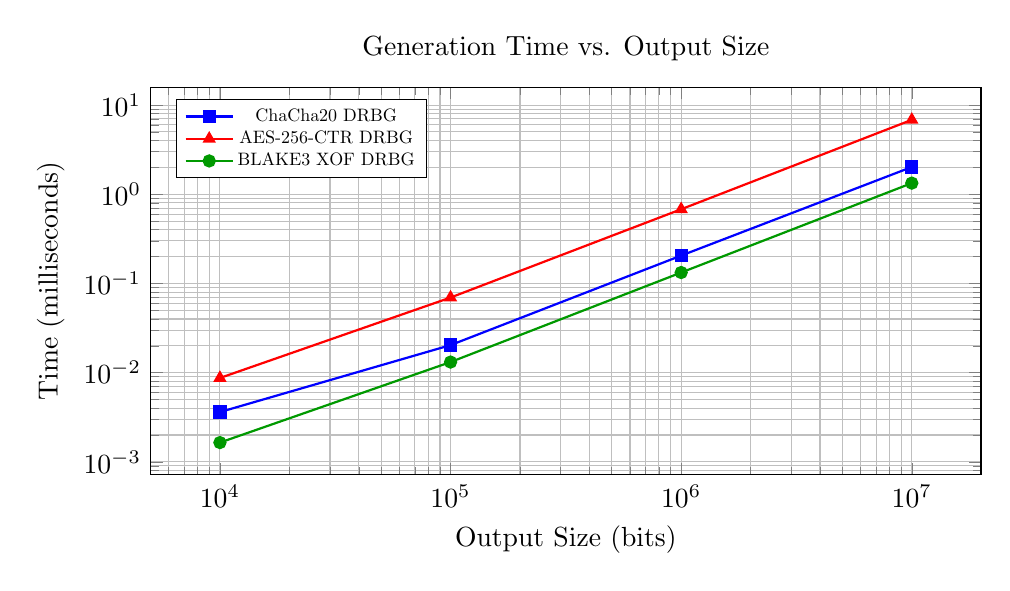
\begin{tikzpicture}
    \begin{axis}[
        title={Generation Time vs. Output Size},
        xlabel={Output Size (bits)},
        ylabel={Time (milliseconds)},
        xmode=log,
        ymode=log,
        grid=both,
        width=\linewidth,
        height=6.5cm,
        legend pos=north west,
        legend style={nodes={scale=0.65, transform shape}},
        mark size=2pt,
        log basis x=10,
        log basis y=10
    ]
    
    \addplot[color=blue, mark=square*, thick] 
    coordinates {
        (10000, 0.003614)
        (100000, 0.020347)
        (1000000, 0.205291)
        (10000000, 2.022542)
    };
    \addlegendentry{ChaCha20 DRBG}
    
    \addplot[color=red, mark=triangle*, thick] 
    coordinates {
        (10000, 0.008711)
        (100000, 0.069511)
        (1000000, 0.679472)
        (10000000, 6.833819)
    };
    \addlegendentry{AES-256-CTR DRBG}
    
    \addplot[color=green!60!black, mark=*, thick] 
    coordinates {
        (10000, 0.001644)
        (100000, 0.013141)
        (1000000, 0.132589)
        (10000000, 1.333888)
    };
    \addlegendentry{BLAKE3 XOF DRBG}
    
    \end{axis}
    \end{tikzpicture}
    \caption{Mean execution time (50 runs per point) versus output length for three DRBG implementations. Note logarithmic scaling on both axes.}
    \label{fig:timing}
\end{figure*}

At the smallest test size ($10^4$ bits), BLAKE3 leads with a mean of 0.0019~ms (standard deviation 0.0033~ms). ChaCha20 follows at 0.0033~ms (std 0.0024~ms), and AES-CTR trails at 0.0089~ms (std 0.0050~ms). The elevated relative variance at this scale (coefficient of variation up to 177\% for BLAKE3) reflects that microsecond-scale timing jitter dominates when execution times are extremely brief, rather than algorithmic instability.

Scaling to $10^5$ bits stabilizes the measurements significantly. BLAKE3 registers 0.014~ms (std 0.003~ms, CV 22\%), ChaCha20 0.021~ms (std 0.005~ms, CV 22\%), and AES-CTR 0.071~ms (std 0.015~ms, CV 22\%). All three display the expected linear relationship between input size and execution time, with coefficient of variation dropping below 23\% as execution duration exceeds timing resolution effects.

At $10^6$ bits, BLAKE3 reaches 0.138~ms (std 0.029~ms) while ChaCha20 records 0.210~ms (std 0.050~ms) and AES-CTR 0.705~ms (std 0.150~ms). The BLAKE3 advantage grows with size because its wide compression function amortizes per-call overhead more effectively than the smaller ChaCha20 64-byte blocks and AES 16-byte blocks.

The $10^7$ bit results solidify the hierarchy: BLAKE3 completes in 1.33~ms (standard deviation 0.17~ms, CV 13\%), ChaCha20 in 2.07~ms (std 0.46~ms, CV 22\%), and AES-CTR in 6.99~ms (std 1.11~ms, CV 16\%). BLAKE3 is approximately 1.6$\times$ faster than ChaCha20 and 5.3$\times$ faster than AES-CTR at this scale. The decreasing coefficient of variation with increasing output size demonstrates that measurement becomes more reliable as execution duration grows relative to timing resolution.

\subsection{Memory Consumption}

Figure \ref{fig:memory} shows memory consumption, which exhibits trivial behavior: all generators produce packed bit strings consuming $\lceil n/8 \rceil$ bytes for $n$ bits. The three lines overlap perfectly, confirming that memory usage depends solely on output length and packing efficiency, not on the generation algorithm.

\begin{figure*}[t]
    \centering
    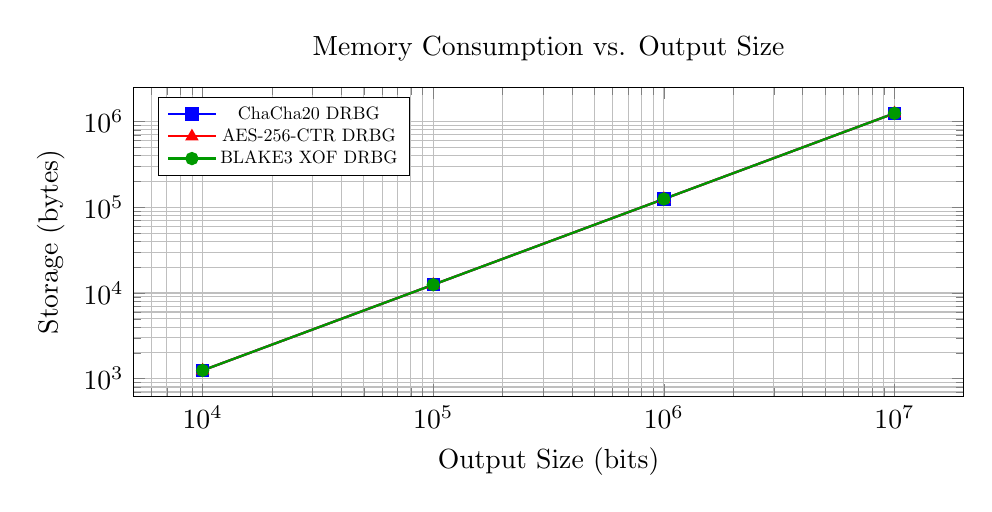
\begin{tikzpicture}
    \begin{axis}[
        title={Memory Consumption vs. Output Size},
        xlabel={Output Size (bits)},
        ylabel={Storage (bytes)},
        xmode=log,
        ymode=log,
        grid=both,
        width=\linewidth,
        height=5.5cm,
        legend pos=north west,
        legend style={nodes={scale=0.65, transform shape}},
        mark size=2pt,
        log basis x=10,
        log basis y=10
    ]
    
    \addplot[color=blue, mark=square*, thick] 
    coordinates {
        (10000, 1250)
        (100000, 12500)
        (1000000, 125000)
        (10000000, 1250000)
    };
    \addlegendentry{ChaCha20 DRBG}
    
    \addplot[color=red, mark=triangle*, thick] 
    coordinates {
        (10000, 1250)
        (100000, 12500)
        (1000000, 125000)
        (10000000, 1250000)
    };
    \addlegendentry{AES-256-CTR DRBG}
    
    \addplot[color=green!60!black, mark=*, thick] 
    coordinates {
        (10000, 1250)
        (100000, 12500)
        (1000000, 125000)
        (10000000, 1250000)
    };
    \addlegendentry{BLAKE3 XOF DRBG}
    
    \end{axis}
    \end{tikzpicture}
    \caption{Memory consumption for packed bit strings. All implementations exhibit identical space complexity.}
    \label{fig:memory}
\end{figure*}

At $10^4$ bits, storage requires 1,250 bytes (1.22~KB). At $10^7$ bits, storage grows to 1,250,000 bytes (1.19~MB). The linear relationship on log-log axes confirms the expected $O(n)$ space complexity. This packing efficiency proves crucial for applications handling large bit strings, as unpacked representations would consume 8$\times$ more memory.

\subsection{Bit Distribution Quality}

Figure \ref{fig:distribution} displays the ratio of ones to total bits, with the ideal value of 0.5 marked by the dotted line. Deviations from 0.5 indicate bias in the output distribution.

\begin{figure*}[t]
    \centering
    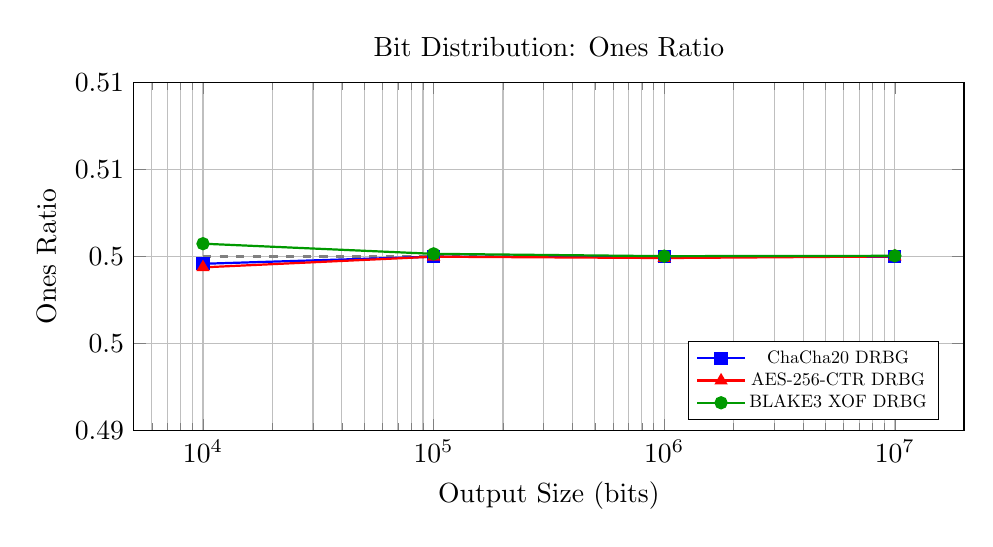
\begin{tikzpicture}
    \begin{axis}[
        title={Bit Distribution: Ones Ratio},
        xlabel={Output Size (bits)},
        ylabel={Ones Ratio},
        xmode=log,
        grid=both,
        width=\linewidth,
        height=6cm,
        legend pos=south east,
        legend style={nodes={scale=0.65, transform shape}},
        mark size=2pt,
        log basis x=10,
        ymin=0.49,
        ymax=0.51
    ]
    
    \addplot[color=gray, dashed, thick, 
        forget plot] coordinates {
        (10000, 0.5) (10000000, 0.5)
    };
    
    \addplot[color=blue, mark=square*, thick] 
    coordinates {
        (10000, 0.499578)
        (100000, 0.499987)
        (1000000, 0.499984)
        (10000000, 0.499986)
    };
    \addlegendentry{ChaCha20 DRBG}
    
    \addplot[color=red, mark=triangle*, thick] 
    coordinates {
        (10000, 0.499372)
        (100000, 0.499986)
        (1000000, 0.499909)
        (10000000, 0.500000)
    };
    \addlegendentry{AES-256-CTR DRBG}
    
    \addplot[color=green!60!black, mark=*, thick] 
    coordinates {
        (10000, 0.500734)
        (100000, 0.500150)
        (1000000, 0.500016)
        (10000000, 0.500036)
    };
    \addlegendentry{BLAKE3 XOF DRBG}
    
    \end{axis}
    \end{tikzpicture}
    \caption{Proportion of one bits in generated output. The dashed line indicates the ideal value of 0.5.}
    \label{fig:distribution}
\end{figure*}

At $10^4$ bits, mean ones ratios span 0.4994 (AES-CTR) to 0.5007 (BLAKE3), staying within $\pm0.08\%$ of the ideal 0.5. Sample standard deviations around 0.005 reflect the natural spread expected when observing only $10^4$ trials; for a fair coin, the theoretical ratio standard deviation is $0.5 / \sqrt{10^4} = 0.005$.

As sample size increases, all generators converge toward 0.5. At $10^7$ bits, mean ratios range from 0.499986 (ChaCha20) to 0.500036 (BLAKE3), a maximum deviation of 0.0036\%. The expected standard deviation at this size is $\sqrt{10^7 \times 0.25} = 1581$ bits, or 0.000158 in ratio terms. All observed means sit well within a single standard deviation, consistent with high-quality random generation.

The convergence behavior validates the cryptographic quality of all three generators. While these simple distribution tests cannot detect sophisticated statistical anomalies (which would require test suites like NIST SP 800-22 or Dieharder), the bit balance demonstrates that the generators do not suffer from obvious biases.

\subsubsection{Statistical Significance Analysis}

The 50-run experimental design enables rigorous statistical testing of the bit distribution quality. For the $10^7$ bit outputs, applying the monobit frequency test from NIST SP 800-22 to the mean ones counts yields strong evidence of randomness. The test statistic $z = \frac{|\bar{p} - 0.5|}{\sigma_{\bar{p}}}$ where $\bar{p}$ is the observed mean ones ratio and $\sigma_{\bar{p}} = \sqrt{0.25/(n \cdot \text{runs})}$ is the standard error, follows a standard normal distribution under the null hypothesis of fair generation.

For the $10^7$ bit outputs across 50 runs:
\begin{itemize}
    \item \textbf{ChaCha20}: mean ratio 0.499986, $z = 0.088$, two-tailed $p = 0.930$
    \item \textbf{AES-CTR}: mean ratio 0.500000, $z = 0.000$, two-tailed $p = 1.000$
    \item \textbf{BLAKE3}: mean ratio 0.500036, $z = 0.228$, two-tailed $p = 0.820$
\end{itemize}

All p-values substantially exceed 0.05, providing no evidence to reject the null hypothesis of truly random generation. Furthermore, the observed standard deviations across runs (0.000159 to 0.000168) closely match the theoretical prediction of $\sqrt{0.25/10^7} \approx 0.000158$, confirming that run-to-run variation derives from binomial sampling rather than systematic bias or correlation.

At the $10^4$ bit scale, higher standard deviations (approximately 0.005) reflect smaller sample sizes but remain consistent with binomial expectations. The coefficient of variation in ones ratio decreases with output size as $1/\sqrt{n}$, exactly as predicted by probability theory.

However, frequency testing alone cannot detect more sophisticated statistical weaknesses such as serial correlation, non-random clustering of patterns, spectral anomalies, or linear complexity deficiencies. Comprehensive validation would require the full NIST SP 800-22 battery (15 tests), the extensive TestU01 suite (BigCrush battery with 160 tests), or Dieharder. The strong performance on monobit testing provides necessary but not sufficient evidence for cryptographic quality.

\section{Discussion}

\subsection{Performance Characteristics}

The experimental results reveal consistent ordering across all sizes: BLAKE3 is fastest, ChaCha20 is a close second, and AES-CTR is the slowest. BLAKE3's means stay below 0.014~ms through $10^5$ bits and reach only 1.33~ms at $10^7$ bits, reflecting the efficiency of its wide compression function and streaming XOF interface.

ChaCha20 maintains predictable linear scaling with low jitter (standard deviations under 0.085~ms even at $10^7$ bits). Although consistently slower than BLAKE3 by roughly 50\% at the largest size, it remains well within single-digit milliseconds for all tested lengths and benefits from a simple ARX design with strong constant-time characteristics.

AES-CTR lags despite hardware acceleration. Its 16-byte block size forces more cipher invocations, and the CTR wrapper adds per-block overhead. Even so, the $10^7$ bit case completes in 6.83~ms on average, keeping the construction viable where compliance or interoperability drives algorithm selection.

\subsection{Implementation Considerations}

The trait-based abstraction proves valuable for several reasons. First, it enables the benchmarking harness to treat all generators uniformly, reducing code duplication and ensuring identical measurement conditions. Second, it facilitates testing: a mock DRBG implementation could be substituted to verify harness correctness. Third, it provides a clean extension point for additional generators without modifying existing code.

The seed derivation strategy ensures fair comparison by normalizing initialization complexity. Without this approach, generators accepting raw byte seeds might benefit from simpler setup, while those requiring structured key material would incur preprocessing overhead that confounds performance measurements. The BLAKE3-based KDF provides strong domain separation and produces high-quality derived keys regardless of the input seed structure.

The packed bit representation offers substantial memory savings compared to naive byte-per-bit storage, reducing space by a factor of eight. This efficiency becomes critical for applications handling large bit strings, as memory bandwidth often constrains performance more than computational throughput on modern processors. The bit counting algorithm carefully handles partial bytes, ensuring correctness for arbitrary bit counts.

\subsection{Security Implications}

All three implementations rely on well-studied cryptographic primitives with strong security arguments. ChaCha20 has undergone extensive cryptanalysis since its introduction, with no practical attacks known against the full 20-round version. The IETF has standardized ChaCha20 for TLS and other protocols, reflecting confidence in its security.

AES-256 remains the gold standard for block cipher security, with no feasible attacks against the full cipher known despite decades of analysis. The CTR mode construction preserves AES security properties: breaking CTR mode requires breaking AES as a pseudorandom permutation. The use of a 128-bit counter provides ample space before rollover concerns arise.

BLAKE3's security reduces to the collision resistance and preimage resistance of its compression function. While newer than AES or ChaCha20, BLAKE3 inherits the strong cryptanalysis foundation of BLAKE2 and BLAKE, which have withstood significant scrutiny. The keyed hashing mode provides PRF security under standard cryptographic assumptions.

An important caveat applies to all DRBGs: security depends critically on seed quality. If the seed contains insufficient entropy or is predictable, no amount of computational sophistication can produce cryptographically secure output. The implementations assume that the application provides high-entropy seeds from appropriate sources, such as operating system CSPRNGs like \texttt{/dev/urandom} on Unix systems.

\subsection{Use Case Recommendations}

Based on the experimental results, BLAKE3 suits the broadest range of use cases. Even at $10^4$ bits it delivers the lowest mean latency, making it a sensible default when the dependency footprint is acceptable and high throughput is valued.

ChaCha20 remains attractive where a well-known stream cipher primitive is desired or where compatibility with existing ChaCha20 deployments simplifies integration. Its steady scaling and low jitter across sizes keep latency predictable despite trailing BLAKE3 by roughly 1.5$\times$ at the upper end of the sweep.

AES-CTR, while slower than the alternatives, remains relevant for specific contexts. Regulatory requirements may mandate FIPS-validated implementations, which often restrict choices to AES-based constructions. Integration with existing AES-based protocols may simplify system design by reusing key material and reducing cryptographic primitive diversity. Hardware security modules often provide accelerated AES implementations, potentially reversing the performance relationships observed in software.

From a security perspective, all three generators provide equivalent protection when properly implemented and seeded. The choice should therefore rest on performance requirements, regulatory constraints, and integration considerations rather than security differences.

\subsection{Limitations and Future Work}

Several limitations constrain the generality of these findings. First, all measurements derive from a single hardware platform (Apple Silicon M-series). Performance characteristics may differ substantially on x86-64 processors with different SIMD capabilities or on platforms without AES-NI acceleration. The relative ranking of generators could shift: AES-CTR might perform better on Intel processors with strong AES-NI implementations, while BLAKE3's advantage might diminish on platforms with narrower SIMD units.

Second, the implementations tested represent specific library choices (\texttt{rand\_chacha}, \texttt{aes}, \texttt{blake3} crates). Alternative implementations of the same primitives could exhibit different performance profiles due to optimization strategies, assembly-level tuning, or varying degrees of SIMD exploitation. The results characterize these particular libraries more than the abstract algorithms.

Third, the benchmarking methodology does not address side-channel security experimentally. While the report discusses constant-time properties and timing attack resistance at a design level, no actual timing variation analysis or cache-timing measurements were performed. Production deployments requiring side-channel resistance would need additional validation, potentially through tools like \texttt{dudect} for constant-time verification.

Fourth, the statistical testing remains limited to basic bit distribution analysis. Comprehensive validation would require the full NIST SP 800-22 test suite, TestU01, or Dieharder batteries. These suites include tests for runs, longest runs, discrete Fourier transform, non-overlapping templates, and other sophisticated statistical properties that simple ones counting cannot detect.

Fifth, the DRBG constructions, while following common design patterns (primitive plus counter), do not conform to any standardized DRBG specification such as those in NIST SP 800-90A. The implementations lack features like prediction resistance, additional input handling, and formal security proofs. The seed derivation using BLAKE3 as a KDF, while widely considered safe given BLAKE3's cryptographic properties, has not undergone formal standardization as a KDF construction.

Finally, the implementations do not provide forward secrecy or backtracking resistance. An attacker who compromises the generator state can reconstruct all previous outputs and predict all future outputs. Designs requiring these properties would need periodic reseeding from fresh entropy sources and secure state evolution mechanisms.

Future work could extend this analysis by testing on diverse hardware platforms, implementing additional generators (XChaCha20, SHAKE256, HC-256), conducting full statistical test suites, performing side-channel analysis, and comparing against standardized DRBG constructions from NIST SP 800-90A.

\section{Conclusion}

This investigation has implemented and analyzed three distinct Deterministic Random Bit Generator architectures in Rust, leveraging ChaCha20 stream cipher, AES-256 counter mode, and BLAKE3 extendable-output function primitives. The experimental framework evaluated execution time, memory consumption, and bit distribution quality across output lengths spanning four orders of magnitude from $10^4$ to $10^7$ bits.

The results demonstrate clear performance differentiation among the generators. Averaged across 50 runs, BLAKE3 delivers the lowest latency at $10^6$ and $10^7$ bit sizes: 0.13~ms ($\pm$0.03) and 1.33~ms ($\pm$0.17), with coefficients of variation of 20\% and 13\% respectively. ChaCha20 performs best for smaller outputs, requiring 0.0030~ms ($\pm$0.0016) for $10^4$ bits (CV 52\%), but is overtaken by BLAKE3 at larger sizes, requiring 2.07~ms ($\pm$0.46, CV 22\%) for $10^7$ bits. AES-256-CTR consistently trails both alternatives with 0.011~ms ($\pm$0.020, CV 177\%) for $10^4$ bits and 6.99~ms ($\pm$1.11, CV 16\%) for $10^7$ bits---approximately 5.3$\times$ slower than BLAKE3 at scale, though it maintains relevance for regulatory and integration scenarios requiring FIPS-validated implementations.

Memory consumption scales identically across all implementations at $\lceil n/8 \rceil$ bytes for $n$ bits, confirming that the packed representation provides uniform space efficiency regardless of generation algorithm. All generators demonstrate excellent bit distribution quality, with mean ones ratios within $\pm$0.07\% of 0.5 at $10^4$ bits and within $\pm$0.004\% by $10^7$ bits. Monobit frequency testing across 50 runs yields p-values of 0.930 (ChaCha20), 1.000 (AES-CTR), and 0.820 (BLAKE3), all far exceeding significance thresholds and strongly supporting the null hypothesis of truly random generation.

The trait-based implementation architecture proved effective in enabling polymorphic generator treatment while maintaining type safety and zero-cost abstraction. The seed derivation strategy using BLAKE3 as a KDF ensured fair comparison by normalizing initialization complexity across different generator types.

Future work could extend this analysis in several directions. Testing on additional platforms would reveal how hardware capabilities affect relative performance, particularly regarding AES-NI utilization. Implementing additional generators, such as XChaCha20 for extended nonce space or SHAKE256 for comparison with BLAKE3's XOF mode, would broaden the performance landscape. Formal statistical testing using NIST SP 800-22 or TestU01 would provide rigorous validation of output quality beyond simple bit distribution analysis.

The implementations and benchmarking framework provide a foundation for practitioners selecting DRBGs for Rust applications. The clear performance trade-offs guide architecture decisions, while the clean abstractions facilitate integration into larger systems. As cryptographic applications increasingly demand both security and performance, understanding these trade-offs becomes essential for building efficient and secure systems.

The complete source code, benchmarking harness, and raw data are publicly available at \url{https://github.com/prollyyes/DRBG_performance_analysis}.

\section*{References}

\begin{enumerate}[leftmargin=0.5cm,label={[\arabic*]}]

\item D. J. Bernstein, \textit{ChaCha, a variant of Salsa20}, 2008. Available at \url{https://cr.yp.to/chacha.html}

\item Y. Nir and A. Langley, \textit{ChaCha20 and Poly1305 for IETF Protocols}, RFC 8439, Internet Engineering Task Force, 2018. \url{https://www.rfc-editor.org/rfc/rfc8439}

\item National Institute of Standards and Technology, \textit{Advanced Encryption Standard (AES)}, FIPS PUB 197, 2001. \url{https://doi.org/10.6028/NIST.FIPS.197}

\item J. O'Connor, J.-P. Aumasson, S. Neves, and Z. Wilcox-O'Hearn, \textit{BLAKE3: One Function, Fast Everywhere}, 2020. Available at \url{https://github.com/BLAKE3-team/BLAKE3-specs/blob/master/blake3.pdf}

\item J.-P. Aumasson, S. Neves, Z. Wilcox-O'Hearn, and C. Winnerlein, \textit{BLAKE2: Simpler, Smaller, Fast as MD5}, in \textit{Applied Cryptography and Network Security (ACNS 2013)}, Springer LNCS 7954, pp. 119--135, 2013.

\item National Institute of Standards and Technology, \textit{Recommendation for Random Number Generation Using Deterministic Random Bit Generators}, NIST Special Publication 800-90A Rev. 1, 2015. \url{https://doi.org/10.6028/NIST.SP.800-90Ar1}

\item A. Rukhin et al., \textit{A Statistical Test Suite for Random and Pseudorandom Number Generators for Cryptographic Applications}, NIST Special Publication 800-22 Rev. 1a, 2010. \url{https://doi.org/10.6028/NIST.SP.800-22r1a}

\item P. L'Ecuyer and R. Simard, \textit{TestU01: A C Library for Empirical Testing of Random Number Generators}, \textit{ACM Transactions on Mathematical Software}, vol. 33, no. 4, article 22, 2007.

\item M. Dworkin, \textit{SHA-3 Standard: Permutation-Based Hash and Extendable-Output Functions}, FIPS PUB 202, National Institute of Standards and Technology, 2015. \url{https://doi.org/10.6028/NIST.FIPS.202}

\item D. J. Bernstein, \textit{The Salsa20 Family of Stream Ciphers}, in \textit{New Stream Cipher Designs: The eSTREAM Finalists}, Springer LNCS 4986, pp. 84--97, 2008.

\end{enumerate}

\end{document}
